\section{Cloud Computing}
\label{sec:Cloud_Computing}

Outsourcing IT infrastructure and services to third parties,
rather than maintaining them in-house, has gained popularity as a cost-effective and flexible solution for businesses.
It allows for reduced upfront costs and increased scalability. \footcite{armbrustCloudsBerkeleyView}

It has become especially popular in form of multi tenant data centers, which are able to provide services to many customers.
This ability to share the costs burden of the infrastructure amongst their customers, making use of the economies of scale
has lead to the rise of the three main cloud providers, Amazon Web Services, Microsoft Azure and Google Cloud Platform\footcite{InfographicAmazonMaintains2024}.

These multi tenant data centers need to guarantee the isolation of hardware and software resources between the different customers,
as highly sensitive, valuable, and mission critical data is stored and processed in these data centers.

While this need has existed before the advent of the cloud computing business model,
as user isolation is a fundamental requirement of any multi-user system,
the need for isolation has become more important since number of customers and the amount of data stored and processed has increased significantly.
This has led to the continual development of virtualization and containerization technologies,
which are used to provide the necessary isolation between the different customers\footcite{randalIdealRealRevisiting2021}.

The two main technologies used to provide these isolated environments are virtualization and containerization.
What they are and how they work will be discussed in the following sections.

\subsection{Virtualization and Isolation}
\label{sec:virtualization}

The differentiating factor of \ac{VM}s is that they are at their core hardware emulators.
They consist of a \gls{host} \ac{OS}, a so called hypervisor and one or more \gls{guest} \ac{OS},
including their dedicated virtual resources like \ac{CPU}, memory, storage, and network interfaces\footcite{gotoKernelbasedVirtualMachine2011}.

This does not only provide isolation between the processes running on the different \gls{guest} \ac{OS}s,
but also enables the users and developers to emulate hardware architectures and run different \ac{OS}s than the \gls{host} \ac{OS}


In figure \ref{fig:full_virtualization} the different layers of a full virtualization setup are shown.
The hardware layer is the actual hardware, which is used to run the \ac{OS} and the hypervisor.

The Hypervisor is a software layer which is responsible for the management of the different \ac{VM}s,
while it may be a separate piece of software, it can also be tightly integrated into the \ac{OS} itself
and is then called a type 1 hypervisor, while a hypervisor running on top of an \ac{OS} is called a type 2 hypervisor\footcite{awsTypeVsType}.

\begin{figure}[ht!]
    \vspace{0.5cm}
    \centering
    \scalebox{0.75}{
        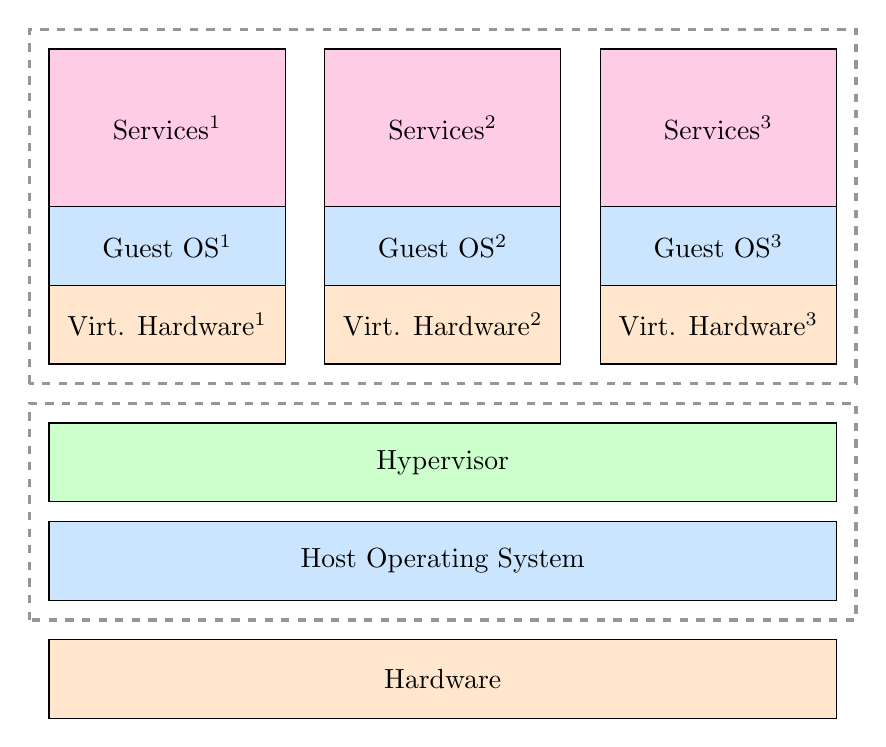
\begin{tikzpicture}
            % Define the colors
            \definecolor{hardwarecolor}{RGB}{255, 230, 204}
            \definecolor{oscolor}{RGB}{204, 229, 255}
            \definecolor{hypervisorcolor}{RGB}{204, 255, 204}
            \definecolor{vmcolor}{RGB}{255, 204, 229}
            \definecolor{dashedlinecolor}{RGB}{150, 150, 150}

            % Draw the Hardware layer
            \filldraw[fill=hardwarecolor, draw=black] (0,0) rectangle (10,1) node[pos=.5] {Hardware};

            % Draw the Host Operating System layer
            \filldraw[fill=oscolor, draw=black] (0,1.5) rectangle (10,2.5) node[pos=.5] {Host Operating System};

            % Draw the Hypervisor layer
            \filldraw[fill=hypervisorcolor, draw=black] (0,2.75) rectangle (10, 3.75) node[pos=.5] {Hypervisor};

            % Draw the dashed boundary of the Host and Hypervisor
            \draw[dashed, draw=dashedlinecolor, very thick] (-0.25,1.25) rectangle (10.25,4.0);

            % Draw the Virtual Machines layer
            % VM1
            \filldraw[fill=hardwarecolor, draw=black] (0, 4.5) rectangle (3, 5.5) node[pos=.5] {Virt. Hardware\textsuperscript{1}};
            \filldraw[fill=oscolor, draw=black] (0, 5.5) rectangle (3, 6.5) node[pos=.5] {Guest OS\textsuperscript{1}};
            \filldraw[fill=vmcolor, draw=black] (0, 6.5) rectangle (3, 8.5) node[pos=.5] {Services\textsuperscript{1}};
            % VM2
            \filldraw[fill=hardwarecolor, draw=black] (3.5, 4.5) rectangle (6.5, 5.5) node[pos=.5] {Virt. Hardware\textsuperscript{2}};
            \filldraw[fill=oscolor, draw=black] (3.5, 5.5) rectangle (6.5, 6.5) node[pos=.5] {Guest OS\textsuperscript{2}};
            \filldraw[fill=vmcolor, draw=black] (3.5, 6.5) rectangle (6.5, 8.5) node[pos=.5] {Services\textsuperscript{2}};
            % VM3
            \filldraw[fill=hardwarecolor, draw=black] (7, 4.5) rectangle (10, 5.5) node[pos=.5] {Virt. Hardware\textsuperscript{3}};
            \filldraw[fill=oscolor, draw=black] (7, 5.5) rectangle (10, 6.5) node[pos=.5] {Guest OS\textsuperscript{3}};
            \filldraw[fill=vmcolor, draw=black] (7, 6.5) rectangle (10, 8.5) node[pos=.5] {Services\textsuperscript{3}};

            % Draw the dashed boundary of the Virtual Machines
            \draw[dashed, draw=dashedlinecolor, very thick] (-0.25,4.25) rectangle (10.25,8.75);

        \end{tikzpicture}
    }
    \caption{Full Virtualization}
    \label{fig:full_virtualization}
\end{figure}

While virtualization is a powerful tool, it is not without its drawbacks, as the overhead of the emulation of an entire hardware stack is a significant performance hit,
which is why \ac{KVM} and Xen have been developed. They are able to pass through instructions directly to \gls{host}s hardware.

Features like \gls{VT-d}, \gls{virtio} and \gls{EPT} are used to respectively pass through \ac{CPU} instructions, network/storage interfaces and memory management to the hardware,
if the hardware supports these features.
But if the hardware does not support these features, the hypervisor will fall back to emulate the needed hardware making it support a wider range of hardware,
but at the cost of performance\footcite{barhamXenArtVirtualization2003}.


\subsection{Containerization}
\label{sec:containerization}

With the need for isolated environments and the economic desire for a more efficient use of resources,
the next logical step was to create a solution which trades the flexibility of virtualization for the
performance of executing \ac{CPU} instructions native to the \gls{host} hardware\footcite{ercegAnotherBriefHistory2022}.

This gap was gradually filled by the development of containerization technologies in the Linux kernel,
by way of giving the \gls{host} \ac{OS} the ability to “jail” processes and denying them to interact with other processes and the \gls{host} \ac{OS}.
This enables the \gls{host} \ac{OS} to run multiple isolated environments, which are called containers,
with close to native performance. \footcite{randalIdealRealRevisiting2021}

The downside of this approach is the strong dependency on the \gls{host}s kernel,
which means that all the containers are bound to its architecture and may not use features of newer kernels,
or legacy features of older kernels\footcite{kovacsComparisonDifferentLinux2017}.

\begin{figure}[ht!]
    \vspace{0.5cm}
    \centering
    \scalebox{0.75}{
        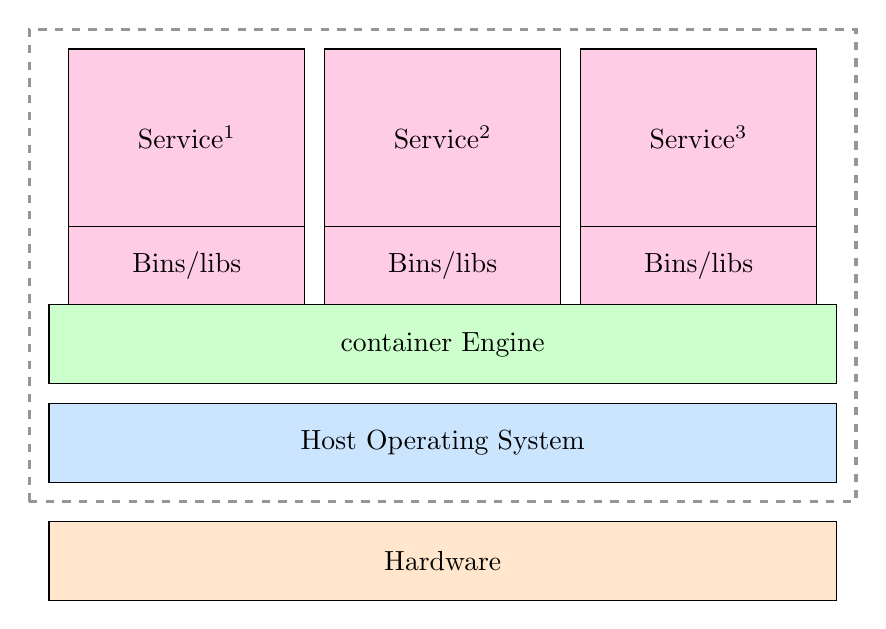
\begin{tikzpicture}
            % Define the colors
            \definecolor{hardwarecolor}{RGB}{255, 230, 204}
            \definecolor{oscolor}{RGB}{204, 229, 255}
            \definecolor{hypervisorcolor}{RGB}{204, 255, 204}
            \definecolor{containercolor}{RGB}{255, 204, 229}
            \definecolor{dashedlinecolor}{RGB}{150, 150, 150}

            % \definecolor{hardwarecolor}{RGB}{217, 224, 189} % Pale yellow
            % \definecolor{oscolor}{RGB}{236, 219, 230} % Lavender
            % \definecolor{hypervisorcolor}{RGB}{185, 218, 247} % Light blue
            % \definecolor{containercolor}{RGB}{204, 247, 220} % Light green
            % \definecolor{dashedlinecolor}{RGB}{255, 235, 204} % Light orange

            % Draw the Hardware layer
            \filldraw[fill=hardwarecolor, draw=black] (0,0) rectangle (10,1) node[pos=.5] {Hardware};

            % Draw the Host Operating System layer
            \filldraw[fill=oscolor, draw=black] (0,1.5) rectangle (10,2.5) node[pos=.5] {Host Operating System};

            % Draw the container Engine layer
            \filldraw[fill=hypervisorcolor, draw=black] (0,2.75) rectangle (10, 3.75) node[pos=.5] {container Engine};

            % Draw the containers layer
            % container1
            \filldraw[fill=containercolor, draw=black] (0.25,  3.75) rectangle (3.25,  4.75) node[pos=.5] {Bins/libs};
            \filldraw[fill=containercolor, draw=black] (0.25,  4.75) rectangle (3.25, 7) node[pos=.5] {Service\textsuperscript{1}};
            % container2
            \filldraw[fill=containercolor, draw=black] (3.5,  3.75) rectangle (6.5,  4.75) node[pos=.5] {Bins/libs};
            \filldraw[fill=containercolor, draw=black] (3.5,  4.75) rectangle (6.5, 7) node[pos=.5] {Service\textsuperscript{2}};
            % container3
            \filldraw[fill=containercolor, draw=black] (6.75,  3.75) rectangle (9.75,  4.75) node[pos=.5] {Bins/libs};
            \filldraw[fill=containercolor, draw=black] (6.75,  4.75) rectangle (9.75, 7) node[pos=.5] {Service\textsuperscript{3}};
            % Draw the dashed boundary of the Host and containers
            \draw[dashed, draw=dashedlinecolor, very thick] (-0.25,1.25) rectangle (10.25,7.25);

        \end{tikzpicture}
    }
    \caption{Containerization}
    \label{fig:containerization}
\end{figure}

In figure \ref{fig:containerization}, a containerization setup is depicted, which includes the hardware,
the \gls{host} \ac{OS}, and the container engine.
The container engine is responsible for managing the containers and the resources they use as well as providing a unified way to interact with the containers.

The emergence of containerization was more of a gradual process than a single release of a new technology,
but the three most important steps in this process were the introduction of the chroot system call,
the introduction of namespaces and the introduction of c-groups, which will be discussed in the following sections.

\subsubsection{Chroot}

The first major step towards process isolation was the introduction of the chroot system call in the 7th edition of Unix and later in the 4.0BSD release,
which was further developed to the chroot jail
These jails where used as am security tool to protect the larger system in \textit{BSD},
this sentiment was not applied when Linux adopted the chroot system call\footcite{bernsteinContainersCloudLXC2014}

While not technically being considered a security feature, as it was not designed to be inherently secure, and therefore is easy to circumvent\footcite{linux-manualpageChrootLinuxManual},
it does provide a way to isolate processes from the rest of the system.
As changing the \gls{root_fs} directory of a process and its children to an arbitrary directory, results in them considering this directory as the \gls{root_fs} of the file system.

This prevents a given process effectively from reaching outside this boundary, as it is unable to access files outside the new \gls{root_fs} directory.
Linux works under the paradigm  "everything is a file”, which means that everything on the system is represented within the file system,
be it a process, a network interface or a block device.
So if the process is unable to access the file, it is unable to access the resource.
This is useful for running untested code which is not suspected to be actively malicious, or for providing a restricted environment for a process to run in.

While some consider \textit{chroot} the first step towards containerization, some argue \footcite{randalIdealRealRevisiting2021} that the true origin might be attributed to the  “process capabilities” function,
which allowed for the limitation of process resource utilization and permissions, this is a key feature of containerization, but as they fell out of favor after the advent of virtualization, we will not discuss them further.

\subsubsection{Namespaces}

The central feature of isolation in modern Linux containerization beyond the simple separation of the file system is the use of namespaces.

As the \textit{chroot} command only provides a way to deny access sections of the file system, a process still needs some way to interact with the rest of the system,
for example to access the network or to create new processes it would need access to the \texttt{/proc} file system, undercutting the isolation provided by chroot.
Therefore, a way to provide a process with its own segregated view of the system is needed, which is where namespaces come in\footcite{datadogContainerSecurityFundamentals2023}

Namespaces are a feature of the Linux kernel, which is used to provide isolation between the 6 different classes of kernel resources.
Five of which are so-called privileged namespaces, which require \gls{root_priv} access to create and manage\footcite{217614}.

\pagebreak

The five privileged namespaces are:
\begin{itemize}
    \item \textbf{PID} — Process IDs
    \item \textbf{NET} — Network devices, stacks, ports, etc.
    \item \textbf{IPC} — System V IPC, POSIX message queues
    \item \textbf{MNT} — Mount points
    \item \textbf{UTS} — Hostname and NIS domain name
\end{itemize}

The sixth namespace, the \textbf{User} namespace, is special,
because it can be used by unprivileged users to create containers,
which is not possible with the other namespaces\footcite{priedhorskyCharliecloudUnprivilegedContainers2017}.

Namespaces are applied to all Linux processes, regardless of whether they run in a container or not,
every process has its own view of the system, which is demarcated by the ID of the namespace it is running in.
Processes with the same namespace ID share the same view of the system,
while processes' with different namespaces are totally ignorant of the other processes existence and influence on the system\footcite{michaelkerriskNamespacesOperationPart2013}.


% I already spent way too much time on this graph!!
% todo: Dont touch ever again!!! 

\begin{figure}[!ht]
    \centering
    \vspace{0.5cm}
    \scalebox{0.75}{
        \begin{tikzpicture}[
                every node/.style = {
                        shape=circle,
                        draw,
                        align=center,
                        minimum size=10mm,
                        inner sep=1pt,
                    },
                level/.style={sibling distance=50mm/#1},
                note/.style={rectangle, draw=none, align=left},
                nsnode/.style={circle, draw, align=center, minimum size=10mm, inner sep=1pt}
            ]


            \node[label=right:init] {1}
            child { node {2}
                    child { node (10) [nsnode] {\textcolor{red}{1}(\textcolor{darkgray}{10})}
                            child { node (11) [nsnode] {\textcolor{red}{2}(\textcolor{darkgray}{11})}}
                            child { node (12) [nsnode] {\textcolor{red}{3}(\textcolor{darkgray}{12})}
                                    child { node (13) [nsnode] {\textcolor{red}{4}(\textcolor{darkgray}{13})}}
                                }
                        }
                }
            child { node {3}
                    child { node {4}}
                    child { node {5}
                            child { node (6) [nsnode] {\textcolor{red}{1}(\textcolor{darkgray}{6})}
                                    child {node (7) [nsnode] {\textcolor{red}{2}(\textcolor{darkgray}{7})}}
                                    child {node (8) [nsnode] {\textcolor{red}{3}(\textcolor{darkgray}{8})}
                                            child {node (9) [nsnode] {\textcolor{red}{4}(\textcolor{darkgray}{9})}}
                                        }
                                }
                        }
                };

            \node[draw=red,fit=(6) (7) (8) (9), inner sep=8pt, label={[rotate=90, anchor=south, yshift=-18mm]west:\color{red}Nested PID Namespace}, shape=rectangle] {};

            \node[draw=red,fit=(10) (11) (12) (13), inner sep=8pt, label={[rotate=90, anchor=south, yshift=-16mm]west:\color{red}Nested PID Namespace}, shape=rectangle] {};

        \end{tikzpicture}
    }
    \caption{Namespace isolation\protect\footnotemark}
    \label{fig:pid_namespace_isolation}
\end{figure}
\footnotetext{Modified from \cite{sultanContainerSecurityIssues2019}}


In figure \ref{fig:pid_namespace_isolation} a simple example of the \ac{PID} namespace is shown,
where the processes 1, 2, 3, 4 and 5 are running in the “init” namespace, which is the namespace the \gls{host} \ac{OS} is running in.
The processes 6, 7, 8 and 9 are running in their own nested \ac{PID} namespace, believing to be the only processes on the system.
The same goes for the processes 10, 11, 12 and 13, which also believe to be processes 1, 2, 3 and 4 in their own namespaces.
This results in a hierarchy of namespaces, where the parents are able to see the children, but not the other way around.
So if a process in the “init” namespace were to kill process 1, it would identify it with its true ID of 1 addressing it in the “init” namespace.
But if it wanted to kill within the nested namespace, it can reference the processed with ID 1 of the namespace by using the ID 6
as the internal \ac{PID}s of a namespace are mapped to a different \ac{PID} in the parents namespace\footcite{michaelkerriskNamespacesOperationPart2013}.

\subsubsection{Control groups}
\label{sec:control_groups}

While chroot isolates the file system and namespaces isolate system resources,
a given service might think it is alone on the system and starts to take up all the resources it can get,
filling memory, taking up all the \ac{CPU} time and saturating the network.
To prevent this from happening intentionally or unintentionally, control groups were introduced \footcite{dockerCgroupsNamespacesWhat2015}
for each of the namespaces, so that each process can be limited in all 6 dimensions.

The c-groups have two levels of enforcement for the limitations,
on one hand there is the hard limit, which is an absolute limit,
that if exceeded will result in the process being terminated immediately.
On the other hand there is also the soft limit which lets the process exceed the limit for a certain amount of time.
But if the system is starved for resources, the services which are overstepping the most get killed first\footcite{linuxkernel-docsMemoryResourceController}.

% Interesting side node,
% how do the c-groups enfroce the limitations?
% Cpu limtiations arent done via percentage but core
% If the memory is exeeded there are two enforcement levels,
% either the process is terminated immedatly,
% or, if the system is running out iof memory, the services which are overstepping the most get killed first.
% 
% additionaly its not possible not to use c groups and namespaces, 
% as they are so deeply ingraned in the way the modern linux works.
% therefore not performance can be gained by not running something in a contianer.

% \subsusbsecton{Union Capable File Systems}
% If more pages are needed for the paper, this could be a good topic to expand on.


\subsubsection{Capabilities}

While the namespaces limit what can be seen and interacted with,
and the c-groups limit how much of the resources can be used,
the \textit{capabilities} make sure that the processes are not able to do anything they are not supposed to do.

This need comes from the binary way Linux handles permissions, as either \gls{root_priv} or not \gls{root_priv}.
In the context of containers we need to differentiate between the ultimate power a process may exert within its own namespace,
but the fine-grained control over what a process may modify in the \gls{host} system.

An example for this would be to \gls{host} an Apache server in a container,
in order to expose the web server to the internet, the container needs to be able to bind to a port.
Without \textit{capabilities} feature the container would need to run as \gls{root_priv}, which would pose a security risk,
as the container would be able to do anything the \gls{root_priv} user can do, which is not desirable.

This is where \textit{capabilities} come in.
They are a way to give a process a subset of the \gls{root_priv} users capabilities,
which are needed to perform a certain task, without giving it the full power of the \gls{root_priv} user.

In the case of the Apache server, the process would need the capability to bind to a port, which is the \texttt{CAP\_NET\_BIND\_SERVICE} capability.
\footcite{sultanContainerSecurityIssues2019}



% what happens when a container is started?

% diagram:
% Docker Daemon
% clone( CLONE_NEWIPC | CLONE_NEWNET |
% CLONE_NEW\ac{PID} | CLONE_NEWUTS | CLONE_NEWNEWNS)
% \gls{host}name setup
% rootfs setup
% pivot root
% mount /dev, /proc, /sys
% IP, firewall setup
% execve( Apache2 )

\pagebreak

\subsection{Container Runtimes}

All these major features work to enable the concept of containers,
the coordination of these features is done via the container runtime
which is responsible for the creation, management, and destruction of containers.

\subsubsection{LXC}

The first container runtime was \ac{LXC}, which was developed in 2008 by the Linux kernel community\footcite{jordanwebbLXCLXDDifferent},
it was the first to exclusively use the mainline kernel features to provide isolation and centered around the idea of a “system container”,
a container pretending to be a full \ac{OS}, which is able to run multiple services and applications\footcite{kumarans.PracticalLXCLXD2017}.

\subsubsection{Docker}
\label{sec:docker}
Nowadays, one of the most popular container runtimes is Docker - a high-level container runtime \footcite{vailsheryLeadingContainerizationTechnologies}
focusing on “application containers”, which are used to run a singular service per container.
Docker extends the basis of  \ac{LXC} container runtime by a \ac{AUFS} file system,
as well as further kernel features providing further isolation\footcite{debabContainersRuntimesWar2021}.

The whole Docker project aims to provide a simple and easy to use interface to the underlying containerization technologies,
it administrates the containers through a unified \ac{API}, the docker \gls{daemon}, to which and from where all the communication goes.

It also provides a standard way of predefining environments, by way of the docker image format.
The docker consists of a set of immutable \ac{RO} layers, stacked onto of each other and then combined with a \ac{COW} layer,
these combine to the file system of the container runtime.
While the \ac{RO} layers are shared between different containers and instances, as resources.
the \ac{COW} layer is unique to each container and is used to store the changes made to the file system for this container\footcite{morabitoHypervisorsVsLightweight2015}.

While Docker has become the de facto standard for containerization, it is not without its drawbacks,
as the docker daemon mandates \gls{root_priv} access to run and operate.
This has been considered as undesirable in the \ac{HPC} community\footcite{mujkanovicSurveyAdaptiveContainerization2023} and some consider it to be proving too large of an attack surface\footcite{priedhorskyCharliecloudUnprivilegedContainers2017}.
Several alternatives have been developed, some as a drop-in replacement for the Docker runtime
like \ac{CRI-O} and Podman, while others like Singularity and Charliecloud are designed to be used in the \ac{HPC} community specifically.


% \subsubsection{Singularity}
% does not require root access to run containers, which is a big plus for \ac{HPC} systems, because the administrators are not always willing to give root access to the users.
% if one wants to run root comands in the container one needs to have the root access on the \gls{host} system, which is a big plus for security.
% has its own MPI support, supports infiniband, gpu and excellerator support
% \footcite{priedhorskyCharliecloudUnprivilegedcontainers2017}
% "here are several pminent issues with this approach, the first being compatibility.
%  The software makes use of kernel namespaces that are not deemed stable by multiple prominent distributions of Linux (e.g. no versions of Red Hat Enterprise Linux or compatibles support it), 
% and may not be included in these distributions for the foreseeable future.
%  A closely related issue is one of dependencies" \footcite{kurtzerSingularityScientificcontainers2017}

\subsection{Orchestration}
\label{sec:orchestration}

For now, we have only talked about the creation and management of containers in the scope of a single \gls{host},
but as the containerization effort was driven by Googles need to manage their data centers,
It was always the intention to manage containers in a distributed environment\footcite{vermaLargescaleClusterManagement2015}.

Coordinating the execution, communication and scheduling of containers in a large scale environment is called orchestration,
and has become a key feature for the cloud computing business model, as it allows for a more efficient use of resources than virtualization
and a more secure and flexible way than traditional \ac{HPC} \glsplural{batch system}\footcite{kennyKubernetesHPCAdministration2021} which will be discussed in the \ref{sec:CDA_HPC} section.

The three dominating orchestrations are Kubernetes, Docker Swarm and Mesos,
with Kubernetes being the most popular by a wide margin, with 46\% of companies reporting to use at least one Kubernetes based service
while Swarm and Mesos are used by 11\% and 9\% of companies respectively\footcite{gardenContainerOrchestratorUsage}.
All these tools have a significant feature overlap,
while differing in their internal approach\footcite{truyenComprehensiveFeatureComparison2019}.
As Kubernetes is by far the most popular while having the most in common with the other two,
we will be using it as a reference for the following discussion.

Kubernetes works as a distributed declarative system,
that means that instead of being told what to do, it is told what should be,
and the cluster does its best to make the desired state a reality.


\subsubsection{Kubernetes Basic Concepts}


At the heart of Kubernetes are the \textit{pods}, they are the smallest deployable unit in Kubernetes
and consist of one or more containers, which are always running together as a single unit.

As they share the same namespaces for network and storage, they are able to communicate with each other and share data.
So even the components of Kubernetes itself are containers running as pods on the cluster.
The core functionality of Kubernetes is to manage and schedule these pods on the different \gls{Node}s of the cluster
and to provide them with the necessary resources to run.

The way to interface with the cluster is through providing a \textit{manifest}, a description of a desired state of the cluster,
usually in form of a \acs{YAML} file, which is then submitted to the \textit{API server} of the cluster.
These manifests specify in which way and under which conditions the pods should be running on the cluster,
and the \textit{controller manager} of the cluster is responsible for making sure that the desired state is a reality.

There are several types of controllers which are used, but the most important of which are the \textit{Jobs}, the \textit{Deployments}, \textit{StatefulSets} and \textit{DaemonSets}.


\begin{itemize}
    \item \textbf{Jobs} are one off tasks which are run to completion, similar to a \gls{batch system} job in a \ac{HPC} environment.
    \item \textbf{Deployments} are used to declare a state of the cluster,
          for example that at anytime there should be 3 instances of a web server running, no matter what happens.
    \item \textbf{StatefulSets} as all the containers in the pods are ephemeral, they will not persist their state after they are terminated,
          for this reason a StatefulSet can be used to provide a stable network identity and stable storage for which an instance of a pod can be associated with.
    \item \textbf{DaemonSets} are pods which permanently run on the nodes of the cluster,
          they are used to provide additional interfaces between the clusters nodes and the containers running on them e.g. a network proxy or a monitoring agent.
\end{itemize}

\subsubsection{High Level architecture}
To ensure a controllable environment for the containers to run in and to communicate with each other, a homogeneous substrate
is provided across the different nodes of the cluster, which is the responsibility of the \textit{container runtime} and the \textit{container network interface}.
To keep all these nodes in sync and to provide a unified way to interact with the cluster, the \textit{control plane} which is itself a containers on the cluster.
The high level architecture of Kubernetes is divided into two main parts, the control plane and the nodes,
The control plane is responsible for the coordination of the different nodes and the management of the different resources.
Itself is divided into several \gls{mico-service} like components, which are responsible for the different management tasks.
Just like everything else the services of the containers themselves are containers running on the cluster\footcite{kubernetes-docsKubernetesComponents}.
The cluster may consist of a single node or thousands of nodes, which are responsible for the actual execution of the containers\footcite{kubernetes-docsNodes}.


\begin{figure}[!ht]
    \centering
    \vspace{0.5cm}
    \scalebox{0.85}{
        \begin{tikzpicture}[node distance=1cm and 1.5cm]
            % Commands to change color scheme

            \definecolor{etcdcolor}{RGB}{237, 240, 177} 1
            \definecolor{controlplanecolor}{RGB}{255, 204, 229}
            \definecolor{nodecolor}{RGB}{204, 229, 255}
            \definecolor{clientcolor}{RGB}{204, 255, 204}
            \definecolor{CNIcolor}{RGB}{255, 230, 204}

            \def\nbetcd{3}
            \def\nbapiserver{2}
            \def\nbscheduler{2}
            \def\nbcontroller{2}
            \def\nbnode{3}
            \edef\alletcd{}
            \foreach \i in {1,...,\nbetcd}{
                    \node[draw, fill=etcdcolor] at ($ (360/\nbetcd * \i:0.9) $) (etcd\i) {etcd};
                    \xdef\alletcd{(etcd\i) \alletcd}
                }
            \node[draw,dotted, fit=\alletcd, inner sep=2mm] (etcd) {};

            \foreach \i in {1,...,\nbscheduler}{
                    \node[draw,
                        rotate fit=90,
                        left=of etcd,
                        fill=controlplanecolor,
                        fit=(etcd.north west) (etcd.south west),
                        minimum height=0.7cm,
                        xshift=\i mm,
                        yshift=-\i mm] (scheduler\i) {};
                }
            \node[draw=none, align=center,rotate=90] at (scheduler\nbscheduler) {scheduler};

            \foreach \i in {1,...,\nbcontroller}{
                    \node[draw,
                        rotate fit=90,
                        left=3cm of scheduler1,
                        fill=controlplanecolor,
                        fit=(etcd.north west) (etcd.south west),
                        minimum height=0.7cm,
                        xshift=\i mm,
                        yshift=-\i mm] (controller\i) {};
                }
            \node[align=center,rotate=90] at (controller\nbcontroller) {controller};

            \foreach \i in {1,...,\nbapiserver}{
                    \node[draw,
                        above=of etcd,
                        fill=controlplanecolor,
                        fit=(scheduler1.north east) (controller1.north east) (etcd.north east),
                        minimum height=0.7cm,
                        xshift=\i mm,
                        yshift=\i mm] (apiserver\i) {};
                }
            \node[align=center] at (apiserver\nbapiserver) {apiserver};
            \draw[<->] (etcd.north) -- (etcd.north|-apiserver1.south);


            \node[above right=5cm of apiserver\nbapiserver] (kubelet1) {};
            \foreach \i in {1,...,\nbnode}{
                    \node[draw, fill=controlplanecolor] (kubelet-box\i) at (kubelet\i) {kubelet};
                    \node[draw,below=0.4cm of kubelet\i, fill=CNIcolor] (runtime\i) {runtime};
                    \node[draw,left=0.2cm of runtime\i, fill=controlplanecolor] (proxy\i) {proxy};
                    \node[draw,right=0.2cm of runtime\i, fill=CNIcolor] (CNI\i) {CNI};
                    \node[draw,below=0.9cm of runtime\i,
                        fit=(runtime\i) (CNI\i) (proxy\i),
                        inner sep=0mm, fill=nodecolor] (kernel\i) {};
                    \node[align=center] at (kernel\i) {kernel};
                    \draw[->] (kubelet-box\i) -- (runtime\i.north);
                    \draw[->] (runtime\i) -- (runtime\i|-kernel\i.north);
                    \draw[<-] (CNI\i) -- (CNI\i |- kernel\i.north);
                    \draw[->] (proxy\i) -- (proxy\i |- kernel\i.north);
                    \node[draw,
                        dashed,
                        fit=(kubelet\i) (runtime\i) (CNI\i) (kernel\i),
                        inner sep=2mm,
                        label={\scriptsize{node\i}}]  (node\i) {};
                    \draw[->] (kubelet-box\i.west) -- ++(-2.25cm,0) |- (apiserver\nbapiserver.east);
                    \draw[-] (proxy\i.north) -- ++(0, 0.55);

                    \pgfmathtruncatemacro\nextnode{\i+1}
                    \node[draw=none, below=2.9cm of kubelet\i] (kubelet\nextnode) {};
                }

            \draw[<->] (scheduler\nbscheduler.east) -- (scheduler\nbscheduler.east|-apiserver1.south);
            \draw[<->] (controller\nbscheduler.east) -- (controller\nbscheduler.east|-apiserver1.south);

            \node[draw,
                dashed,
                fit=(etcd) (apiserver1) (apiserver\nbapiserver),
                inner sep=2mm] (controlplane-nodes) {};

            \node[draw,
                above=1cm of apiserver\nbapiserver,
                minimum width=3cm,
                minimum height=0.7cm,
                fill=clientcolor] (client) {Client};
            \draw[<->] (client) -- (apiserver\nbapiserver);

            \coordinate (Start) at ($(CNI1.east)+(0.7cm,0)$);
            \coordinate (End) at ($(CNI\nbnode.east)+(0.7cm,0)$);

            \foreach \i in {1,...,\nbnode}
                {
                    \ifnum\i<\nbnode
                        \pgfmathtruncatemacro\nextNode{\i+1}
                        \draw ($(CNI\i.east)$) -- +(+0.7cm,0) -|  ($(CNI\nextNode.east)+(0.7cm,0)$) -- ($(CNI\nextNode.east)$);
                    \fi
                }

            % Label for the CNI network
            \path (Start) -- (End) node[midway, anchor=south, rotate=-90] {Node-Network};

            %% Stop  using the tikz, you always get lost in the details and never get anything done.
            %% Its just too much fun to play with the details.
        \end{tikzpicture}
    }
    \caption{High Level Architecture\protect\footnotemark}
    \label{fig:high_level_architecture}
\end{figure}

\footnotetext{Modified from \cite{zempashiZempashiKubetraining}}


\textbf{Control Plane}

A state is declared to the system via the unified \ac{API} \texttt{kube-apiserver},
this preferred state is then given to the \texttt{etcd}, a distributed \gls{kv store},
which is used as the \gls{Single source of truth} for the cluster\footcite{nalawalaComprehensiveStudyEtcd2022}.

On a regular basis, the \texttt{kube-controller-manager} checks the actual state of the cluster against the desired state,
if the actual state deviates form the desired state\footcite{kubernetes-docsCloudControllerManager}
the \linebreak
\texttt{kube-controller-manager} will wake the corresponding controller for the resource in question,
which knows what to do to make the actual state match the desired state \footcite{kubernetes-docsControllers}

This woken controller then submits a request to the \texttt{kube-scheduler} via the \ac{API},
which then assigns the task to a node, based on the current scheduling policy\footcite{kubernetes-docsKubernetesScheduler}.

\textbf{Nodes}

On the Side of the clusters nodes, the \texttt{kubelet} is responsible for interfacing with the local container runtime
through the \ac{CRI} and handles the execution of the containers locally on behest of the larger cluster.
Once the kubelet has announced itself to the \texttt{kube-apiserver} the node is ready to run containers.
If the scheduler has assigned a task to the node, the \texttt{kubelet} will check if it
needs to pull the container image from the registry, and then start the container\footcite{kubernetes-docsKubelet}.

The other service running on all nodes is the \ac{CNI}, which is responsible for the networking of the containers.
The \ac{CNI} is a plugin-based system, which allows for the use of different underlying networking solutions,
in order to provide the container with a layer 3 network interfaces and a \ac{IP} address\footcite{thelinuxfoundationCNI}.

The \texttt{kube-proxy} is responsible for regularly checking in with the \texttt{kube-apiserver} and updating the local \ac{IP} tables,
to make sure that the containers are able to communicate with each other and the outside world\footcite{kubernetes-docsKubeproxy}.

The containers themselves are run within a \texttt{Pod}, which is the smallest unit of work in Kubernetes.
While a \texttt{Pod} can consist of as little as a  singular container, the idea is to provide a way to allocate a main container,
in combination with additional supporting containers, which are used to provide additional services to the main container.
An example for this would be a main container running a service which needs to be able to access a database.

The connection to the \ac{DB} instead of hard-coding the service simply calls localhost,
and the support container being a sidecar container, which is working as an easily replaceable proxy to the database.

All this while a third container captures the entire stdout and stderr of the main container and sends it to a log aggregator.

\subsubsection{Networking}
\label{sec:K8sNetworking}

As already mentioned the networking of Kubernetes is quite involved in order to provide the flexibility, isolation, and performance needed for a large scale distributed system.
This is because the containers need to be replaceable on a whim, accessible both from the outside and the inside of the cluster,
but should also all have a unique \ac{IP} address without the need for \gls{NAT}.
This is achieved by abstracting the networking into three different levels, the pod level, the node level and the cluster level.


\begin{figure}[!ht]
    \centering
    \scalebox{0.85}{
        \begin{tikzpicture}[node distance=1cm and 1.5cm]
            \definecolor{nodecolor}{RGB}{204, 229, 255}
            \definecolor{servicenetworkcolor}{RGB}{255, 204, 229}
            \def\nbnode{3} % Number of nodes

            % Assuming a maximum number of pods to calculate node sizes dynamically
            \def\maxpods{3}
            \def\podsize{1cm}


            % Define styles for elements
            \tikzset{
                nodebox/.style={draw, fill=nodecolor, minimum width=3.5cm, minimum height=5cm},
                pod/.style={inner sep=0pt, minimum size=\podsize}
            }

            \foreach \i in {1,...,\nbnode}{
                    % Draw nodes
                    \node[nodebox] (node\i) at (5*\i, 0) {};
                    \node[above=0 of node\i] {Node \i};

                    % Dynamically calculate the number of pods for this example
                    % \pgfmathtruncatemacro\nbpods{random(2,\maxpods)}
                    \pgfmathtruncatemacro\nbpods{\maxpods}

                    % Calculate starting xshift to center pods
                    \pgfmathsetmacro\startxshift{(\podsize - \nbpods*1cm) / 2 - 0.25cm}



                    % Draw pods inside each node equally spaced on the x-axis and centered
                    \foreach \j in {1,...,\nbpods}{
                            % Adjust xshift for each pod
                            \pgfmathsetmacro\currentxshift{\startxshift + (\j-1)*1cm}
                            \node[pod, right=of node\i.west, xshift=\currentxshift, yshift=-1cm] (pod\i\j) {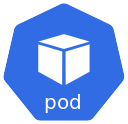
\includegraphics[width=\podsize,height=\podsize]{graphics/k8s_pod.png}};

                        }
                }

            % Sercice network box
            \fill[draw,dashed, fill=servicenetworkcolor, opacity=0.5] ($(node1.north west)+(0.25,-0.25)$) rectangle ($(node\nbnode.mid east)+(-0.25,0)$);

            % Drawing to paralel lines in the the service network box the same length as the pod network line
            \draw ($(node1.north west)+(0.5,-1)$) -- ($(node\nbnode.north east)+(-0.5,-1)$) ;
            \draw ($(node1.north west)+(0.5,-2)$) -- ($(node\nbnode.north east)+(-0.5,-2)$) ;

            \node at ($(node2.north)+(0,-0.75)$) {Service Networks};


            % Draw the node network line dynamically based on nodes
            \coordinate (Start) at ($(node1.south west)+(-0.5cm,-1cm)$);
            \coordinate (End) at ($(node\nbnode.south east)+(0.5cm,-1cm)$);
            \draw (Start) -- (End) node[midway,below] {Node Network};

            % Draw lines from the middle of the nodes to the node network
            \foreach \i in {1,...,\nbnode}{
                    \draw (node\i.south) -- ($(node\i.south)+(0,-1cm)$);
                }

            % Draw the pod network line dynamically based on pods
            \coordinate (PodStart) at ($(pod11.south west)+(0, -0.5cm)$);
            \coordinate (PodEnd) at ($(pod\nbnode\maxpods.south east)+(0,-0.5cm)$);
            \draw (PodStart) -- (PodEnd) node[midway,below] {Pod Network};

            % Draw lines from the bottom of each pod to the pod network
            \foreach \i in {1,...,\nbnode}{
                    \foreach \j in {1,...,\maxpods}{
                            \draw (pod\i\j.south) -- ($(pod\i\j.south)+(0,-0.5cm)$);

                            % Randomly decide whether the pod connects to service network line 1, line 2, or none
                            \pgfmathsetmacro\connectTo{int(random(0,2))} % Generates 0, 1, or 2

                            % Connect to service network line 1
                            \ifnum\connectTo=1
                                \draw (pod\i\j.north) -- ($(pod\i\j.north)+(0,1cm)$);
                            \fi

                            % Connect to service network line 2
                            \ifnum\connectTo=2
                                \draw (pod\i\j.north) -- ($(pod\i\j.north)+(0,2cm)$);
                            \fi
                            % If \connectTo is 0, no line is drawn
                        }
                }

            % Draw encompassing box for the k8s cluster
            \node[draw, dashed, fit=(node1) (node\nbnode) (Start) (End), inner sep=1cm, label=above:Kubernetes Cluster] (cluster) {};

        \end{tikzpicture}
    }
    \caption{Kubernetes Network Diagram\protect\footnotemark}
    \label{abb: k8s_networkdiagramm}
\end{figure}
\footnotetext{Based on: \cite{kubernetes-docsClusterNetworkinga}}


\textbf{Pod level}
At the pod level, the containers share the same network namespace and therefore also the same \ac{IP} address.
The communication between the different containers happens through the loop-back interface,
so that the containers are able to communicate with each by simply calling on their \texttt{localhost} interface.
This is made possible through the \texttt{pause} container, a container in every pod which handles the whole administration
of basic tasks, like  setup  of the namespaces, network interfaces or the killing of \gls{zombies} in the \ac{PID} namespace\footcite{sookocheffGuideKubernetesNetworking2018}.

\textbf{Node level}

Each pod has its own network namespace and its own dedicated \ac{IP} address, which is unique to the pod and is reachable from the entire cluster.
If two pods need to communicate with each other,
each of them \gls{patching} their network interface to the root network namespace via a \texttt{\ac{VETH}} pair.
Now the root network namespace can see the two \texttt{\ac{VETH}} endpoints as two network interfaces,
it can \gls{bridge}  the two interfaces, which allows the two pods to communicate with each other \footcite{sookocheffGuideKubernetesNetworking2018}.


\textbf{Cluster level}

If the pod needs to communicate with another pod on a different node,
the \gls{bridge}ing will fail as the \ac{ARP} will not be able to reach an Ethernet interface on the other node.
If this happens the bridge will forward the packet to the default gateway,
which is the real outwards facing network interface of the node connected to the rest of the network.
The routing of the packets is then handled by the \ac{CNI} plugin, which is responsible for the networking of the clusters nodes.
The \ac{CNI}s job is to provide the containers with a layer 3 network interfaces and an \ac{IP} address,
which is unique to the pod and is reachable from the entire cluster\footcite{laurentbernailleKubeConCloudNativeConNorth2018}.
How they do this is up to the \ac{CNI} plugin itself, as network infrastructure and IP allocation can be very different depending on the underlying infrastructure.
While \ac{CNI} plugins like \texttt{flannel} or \texttt{calico} simply provide flat layer 3 networks,
with external routing. Others like \texttt{DataDog's} custom solutions enable direct pod to pod routing without any layer or bridge in between\footcite{laurentbernailleKubeConCloudNativeConNorth2018}.

\textbf{Services}

A special case in this situation is, if a website, database or any other external interface
is supposed to be able to be accessible under a certain \ac{IP} address permanently.
As the containers are ephemeral so are their \ac{IP} addresses and if the underlying container is replaced the \ac{IP} address will change.
To be able to expose a services running in pods which can be replaced at any time,  Kubernetes provides the concept of the \texttt{Service}.

A \texttt{Service} is a stable \ac{IP} address, which is reachable from the entire cluster, and is used to expose a set of pods to the outside world.
It can be used to expose a single pod, a set of pods or even a set of pods running on different nodes and balance the load between them.
Even when the \ac{IP} address of the pods changes, the \texttt{Service} will still be reachable under the same \ac{IP} address\footcite{velayudhanVisualGuideKubernetes}.

The solution to this problem is to use \texttt{Service}, which works as both a proxy and a load balancer.
The \texttt{Services} have a whole network of their own, neither in the “real” network the nodes are connected to, nor in the pod network.
Unlike the pod network, services don't even have a virtual network interface associated with their IP address.
This would prevent them from being routable if it weren't for the kube-proxy.
Utilizing the IP tables of the nodes, as well as the Netfilter of the Linux kernel,
the kube-proxy is able to reroute packets mid-flight from the service IP to the current IP address of a pod\footcite{betzUnderstandingKubernetesNetworking2022}.
The \texttt{kube-proxies} keeps in sync with the global state of the cluster by regularly checking in with the \texttt{kube-apiserver} and updating their local
routing rules accordingly.

% \textbf{Ingress}

% Here I should talk more about ingress services, but as we specifically are running on a bare metal machine, which doesn not have the 
% capabilities to configure our loadbalancers dynamically, I will for now leave it at that.

% \todo{Ingress}

\subsubsection{Scheduling}

As mentioned above, when Google started to work on the Kubernetes predecessor, the Borg system,
the initial goal was to provide a way to have both their high availability services and their non production jobs,
including large scale batch processing jobs running on the same infrastructure\footcite{abhishekvermaLargescaleClusterManagement2015}.

Therefore, a balance needed was between having a low latency and free resources for the high availability services,
to be able to react to the changing demand of the users, and to be able to run the batch processing jobs which were not as
time or latency sensitive as the high availability services.
So not only does the scheduler need to optimize when to start which pods, but should also take into
account the different priorities of the jobs as well as complex constraints like physical and logical distances of interconnected services,
the availability of the required hardware, or the need to anticipate the future demand of the users\footcite{vermaLargescaleClusterManagement2015}.
Therefore, the scheduler does not only start the pods, but is also able to evict, reschedule and scale the pods according to the current demand of the cluster.

Google's solution to this problem is a highly customizable and flexible scheduling system, which bases its decisions in two steps.

\begin{itemize}
    \item \textbf{Predicates} The predicates are a set of knockout criteria which ideally disqualify a node from being able to run a pod (no capacity, missing important hardware ...)
    \item \textbf{Priorities} The priorities are a set of weighted criteria which are used to rank the remaining nodes, to find the best fit for the pod.
\end{itemize}

Based on these two steps, the state of the cluster and the specific requests of the pod, the scheduler is able
to make a decision whether and where to run the pod\footcite{zivukuInDepthAnalysisKubernetes2023}.
After the decision has been made, the scheduler updates the \texttt{etcd} through the \texttt{kube-apiserver},
with the new state of the cluster.
Then the \texttt{kubelet} on the node is expected to poll the \texttt{kube-apiserver} and to start the pod,
once it has become aware of the new state of the cluster\footcite{kubernetes-docsKubelet}.

Native Kubernetes provide a myriad of different options to influence the schedulers' behavior\footcite{rejibaCustomSchedulingKubernetes2023}.

\begin{itemize}
    \item \textbf{nodeSelector} is a simple binary label matching system. If the node has the required label, the pod can be scheduled on it. This mechanism allows for straightforward restrictions on pod placement based on node labels.
    \item \textbf{Node Affinity} offers a more nuanced approach compared to nodeSelector, allowing specifications of node preferences rather than strict requirements. Pods can still be scheduled even if preferred labels are not found on any node, which makes this a more flexible option than nodeSelector\footcite{kubernetes-docsAssigningPodsNodes}.
    \item \textbf{Inter-pod Affinity/Anti-Affinity} considers the current pod topology for scheduling decisions, aiming to place pods in proximity to or at a distance from each other based on specified criteria. This is beneficial for optimizing network traffic or ensuring high availability by distributing instances of a service across different nodes.
    \item \textbf{Taints and Toleration} work together to ensure that pods are not scheduled onto inappropriate nodes. Taints are applied to nodes and can repel pods that do not have a matching toleration. This is useful if certain nodes have special hardware or are reserved for certain tasks.
\end{itemize}

The Scheduler is not only for starting a pod, but also evicts pods which need to be rescheduled or are not needed anymore.
There are two main reasons why a pod might be evicted, the first is that there is something more important which needs to be run on the node.
This is the so-called \textit{preemption}, which is the act of evicting a lower priority pod to make room for a higher priority pod.
The priority is simply determined by a numerical value associated to a pod, which is then used to rank the pods on the node\footcite{martinezUnderstandingKubernetesEvicted2022}.

The second reason is the so-called \textit{eviction}, which is generally caused by the node running out of resources,
this is called a \textit{node pressure}.
Kubernetes, by way of the kubelets, listens to the resource utilization of the nodes. If a critical threshold is reached,
it will start to evict. The kubelet will make a decision based on the \ac{QoS} class of the pod as well as its \ac{PDB}.

The \ac{QoS} class is a simple way to categorize the pods based on their resource requirements,
they are a manifestation of the soft and hard resource limits of the cgroups already mentioned in section \nameref{sec:control_groups}.
Kubernetes differentiates between the following three classes in order of priority\footcite{matiasnicolettiUnderstandingKubernetesPod2023}:

\begin{enumerate}
    \item \textbf{Guaranteed} pods have both a hard and a soft limit, and are guaranteed to have the resources they need.
    \item \textbf{Burstable} pods have a hard limit, which is higher than the soft limit, and are allowed to burst up to the hard limit.
    \item \textbf{BestEffort} pods have no limits and are allowed to use all the resources of the node, which are not reserved for the system.
\end{enumerate}

If the resource needs can not be easily  estimated, but a hard requirement of a certain number of pods still needs to be met
the \ac{PDB} can be used.
The \ac{PDB} is a way to specify the minimum number of pods of a certain type which need to be running on the cluster.
If a node is running out of resources, the kubelet will check if the eviction of a pod would cause the number of pods of a certain type to fall below the specified number,
and refuse the eviction for that pod\footcite{matiasnicolettiUnderstandingKubernetesPod2023}.

While Kubernetes offers quite a powerful and flexible scheduling system, the user is not limited to use only this system.
Especially for the \ac{HPC} community, the Kubernetes scheduler is not always the best fit, as its design is geared towards the
balance between high availability services and resource utilization, the former of which is not always the main concern in \ac{HPC} environments \footcite{misaleStandardKubernetesScheduling2022}.

Next to the direct modification of the scheduler source code, Kubernetes offers  3 different ways
to introduce custom scheduling logic to the cluster\footcite{rejibaCustomSchedulingKubernetes2023}.
For one there is always the possibility to write a custom scheduler, which is the most flexible way to introduce custom scheduling logic,
and has been done as by the \texttt{Kube-batch} scheduler, which is specifically designed to take into account the needs of the \ac{HPC} community\footcite{kubernetes-docsKubernetesretiredKubebatch2024}.
Alternatively Kubernetes also offers less invasive ways to introduce custom scheduling logic, like the \texttt{Extender API} or the \texttt{Scheduling Framework},
which allow for the extension of the default scheduler, without the need to write a custom scheduler, while providing extensive customization options\footcite{kubernetes-docsSchedulingFramework}.


\pagebreak